% ======================================================================
% Chapter 14: Confinement and Asymptotic Freedom
% Source: R. Gupta, "Introduction to Lattice QCD", arXiv:hep-lat/9807028
% Figures: 10-13; Table 6.
% ======================================================================

\chapter{Confinement and Asymptotic Freedom}

For any theory to provide a successful description of strong interactions
it should simultaneously exhibit the phenomena of confinement at large
distances and asymptotic freedom at short distances. Lattice calculations
support the hypothesis that for non-abelian gauge theories the two domains
are analytically connected, and confinement and asymptotic freedom
coexist. Similary, one way to show that QCD is the correct theory of
strong interactions is that the coupling extracted at various scales (using
experimental data or lattice simulations) is unique in the sense that its
variation with scale is given by the renormalization group. The data for
$\alpha_s$ is reviewed in Section~19. In this section I will discuss what
these statements mean and imply.

\section{Asymptotic Freedom}
\label{sec:asymptotic-freedom}

The term asymptotic freedom implies that the running coupling $g \to 0$ as
the momentum scale of the probe $\mu \to \infty$. This is characterized by
the $\beta$-function
\begin{equation}
  \mu\frac{\partial g}{\partial\mu}
  = -\beta(g) = -(\beta_0 g^3 + \beta_1 g^5 + \ldots)
  \label{eq:beta-fn}
\end{equation}
where $\beta(g)$ is positive for non-abelian gauge groups. In this case
$g = 0$ is a UV stable fixed point of the theory, and about this point the
theory can be analyzed using standard perturbative expansions. This novel
behavior was confirmed by 't~Hooft, Politzer, and by Gross and Wilczek who
showed that the perturbative $\beta$-function satisfies
Eq.~\eqref{eq:beta-fn} [116], i.e., for $N$ colors and $n_f$ active
flavors
\begin{equation}
  \begin{aligned}
    \beta_0 &= \left(\frac{11N - 2n_f}{3}\right)\!/16\pi^2, \\
    \beta_1 &= \left(\frac{34N^2}{3} - \frac{10N n_f}{3}
               - \frac{n_f(N^2-1)}{N}\right)\!/(16\pi^2)^2.
  \end{aligned}
  \label{eq:beta-coeffs}
\end{equation}
These two leading terms in the expansion of $\beta(g)$ are gauge and
regularization scheme invariant. From these it is easy to see that $\beta(g)$
is positive for $n_f < 8$. This result was essential in establishing QCD as
the theory of strong interactions for it explained existing experimental
data which showed that the strength of strong interactions decreases as the
momentum exchanged in a process increases.

Asymptotic freedom, Eq.~\eqref{eq:beta-fn}, implies that QCD dynamically
generates a mass scale. Integrating Eq.~\eqref{eq:beta-fn} from momentum
scale $\mu_1$ to $\mu_2$ with $\mu_2 > \mu_1$ and keeping only the
$\beta_0$ term to simplify the standard calculation, gives
\begin{equation}
  \frac{1}{2\beta_0 g^2(\mu_2)} - \frac{1}{2\beta_0 g^2(\mu_1)}
  = \log\frac{\mu_2}{\mu_1},
  \label{eq:integrate}
\end{equation}
i.e.\ the coupling constant of non-abelian gauge theories depends
logarithmically on the momentum scale of the process. Rewriting
Eq.~\eqref{eq:integrate}
\begin{equation}
  \begin{aligned}
    \frac{1}{2\beta_0 g^2(\mu)} - \log\mu &= \text{constant} \\
    \implies \exp\left(\frac{1}{2\beta_0 g^2(\mu)}\right)
      &= \frac{\mu}{\Lambda_{QCD}} \\
    \implies \alpha_s(\mu) = \frac{g^2(\mu)}{4\pi}
      &= \frac{1}{8\pi\beta_0\log\frac{\mu}{\Lambda_{QCD}}}
  \end{aligned}
  \label{eq:alpha-s}
\end{equation}
introduces $\Lambda_{QCD}$, the invariant scale of the theory with
dimensions of mass. Thus QCD, a theory with a dimensionless coupling
constant and no intrinsic mass scale in the absence of quark masses,
dynamically generates a mass scale. This happens because in order to
specify $g$ one has to also specify a momentum scale at which it is
defined. Extending the above analysis to include $\beta_1$ in
Eq.~\eqref{eq:beta-fn} gives
\begin{equation}
  \Lambda_{QCD} = \lim_{\mu\to\infty}
    \mu \left(\frac{1}{\beta_0 g^2(\mu)}\right)^{\beta_1/2\beta_0^2}
    \exp\left[-\frac{1}{2\beta_0 g^2(\mu)}\right]
    \equiv \mu f_p(g(\mu)) .
  \label{eq:lambda-2loop}
\end{equation}
This 2-loop definition of $\Lambda_{QCD}$ is not unique; the value of
$\Lambda_{QCD}$ depends on the the precise relation between $g$ and $\mu$.
However, once the value of $\Lambda$ is determined in one scheme it can be
related to that in any other perturbative scheme. For example, in the
lattice regularized theory $\Lambda_{lattice}$ is also defined by
Eq.~\eqref{eq:lambda-2loop} but with $\mu$ replaced by $1/a$. Then to
1-loop
\begin{equation}
  \frac{\Lambda_{QCD}}{\Lambda_{lattice}}
    = \mu a \exp\left[-\left(\frac{1}{2\beta_0 g^2(\mu)}
      - \frac{1}{2\beta_0 g^2(a)}\right)\right].
  \label{eq:lambda-ratio}
\end{equation}
In perturbation theory the two coupling constants are related as
\begin{equation}
  g^2(\mu) = g^2(a)\left[1 - \beta_0 g^2(a)\left(\log(\mu a)
    - \log C\right) + O(g^4)\right]
  \label{eq:coupling-rel}
\end{equation}
By substituting Eq.~\eqref{eq:coupling-rel} into Eq.~\eqref{eq:lambda-ratio}
one finds
\begin{equation}
  \Lambda_{QCD} = C\, \Lambda_{lattice}
  \label{eq:lambda-C}
\end{equation}
i.e.\ the two constants, $\Lambda_{QCD}$ and $\Lambda_{lattice}$, are
related by a multiplicative constant. To calculate $C$ requires knowing the
finite part of the coupling

\begin{table}[htbp]
  \centering
  \begin{tabular}{lccccc}
    \toprule
    $n_f$ & 0 & 1 & 2 & 3 & 4 \\
    \midrule
    $\Lambda_{\overline{MS}}/\Lambda_{latt}$ & 28.8 & 34.0 & 41.1 & 51.0 & 65.5 \\
    $\Lambda_{\overline{MOM}}/\Lambda_{latt}$ & 83.4 & 89.4 & 96.7 & 105.8 & 117.4 \\
    \bottomrule
  \end{tabular}
  \caption{The relation between $\Lambda_{\overline{MOM}}$ and
    $\Lambda_{\overline{MS}}$ and $\Lambda_{latt}$ as a function of the
    number of active flavors. The results for
    $\Lambda_{\overline{MOM}}/\Lambda_{latt}$ with $g$ defined by the
    triple gluon vertex are in Feynman gauge.}
  \label{tab:6}
\end{table}

constant renormalization to 1-loop in both the lattice and continuum
regularization schemes [117,36]. The results are listed in
Table~\ref{tab:6} for $\Lambda_{\overline{MOM}}$ and
$\Lambda_{\overline{MS}}$. It is important to note that even though the
above definition and estimate of $\Lambda_{QCD}$ is made using perturbation
theory, it is intrinsically a non-perturbative quantity.

All dimensionful quantities in lattice simulations are measured in units of
the lattice spacing, for example one measures $M a$ and not $M$. Such
dimensionless quantities vary with $g$ as
\begin{equation}
  M_i a = c_i f_i(g) \equiv c_i \Lambda_i^{\mathrm{non}\text{-}\mathrm{pert}} a .
  \label{eq:scaling-ma}
\end{equation}
where the $c_i$ are constants representing the continuum value and $f_i$ are
scaling functions. Lattice correlation lengths $\xi_i \equiv 1/M_i a$
diverge as the fixed point at $g = 0$ is approached. This divergence is an
artifact---it is the unit of measurement $a$ that is going to zero and not
$M_i$. This is precisely what one wants to have happen to get rid of the
scaffold (lattice) erected to regularize the theory. Non-perturbative
renormalization consists of taking the continuum limit holding some
physical quantity $M_i$ fixed while allowing $a \to 0$ according to
$f_i(g)$. The particular quantity $M_i$ (string tension, or nucleon mass,
etc.) held fixed defines the renormalization condition, and the constraint
between $a$ and $g$ is the scaling relation.

\begin{itemize}
  \item \textit{Scaling:} The hypothesis of scaling is that all $f_i(g)$
    converge to a universal scaling function $f(g) = \Lambda^{\mathrm{non}\text{-}\mathrm{pert}} a$.
    The renormalization condition is then independent of the state used to
    define it. For $g < g_{scaling}$ each lattice quantity is characterized
    by the non-perturbative number $c_i$ and all dimensionless ratios of
    physical quantities are independent of $g$.
  \item \textit{Asymptotic Scaling:} Close to the fixed point at $g = 0$,
    perturbation theory is apposite and all $f_i(g) \to f_{pert}(g) \to
    \Lambda_{QCD} a$.
\end{itemize}

Lattice simulations, therefore, provide continuum results to within some
error tolerance from simulations done in a neighborhood of $g = 0$. In this
region scaling holds. For a fixed error criteria, the extent of this scaling
window can be enlarged by improving the action and operators as discussed
in Section~8. For simulations done outside the
scaling window it is imperative that a reliable extrapolation to $a = 0$ be
done. Obviously, one way to get an upper bound on the errors is to compare
the measured scaling function with $f_{pert}(g)$. The good news is that
simulations in the past few years show that corrections to scaling can be
reduced to a few percent level for lattice spacings with
$5 \lesssim \xi/a < 10$ (where $\xi/a = 1/(\sqrt{\sigma}\,a)$). This
corresponds to $2 \lesssim 1/a \lesssim 4$~GeV. Consequently, realistic
results with physical light quarks can be obtained on lattices of side
$\sim 75 - 150$, and for many quantities, like those involving the heavy
quarks, much smaller lattices are sufficient. The goal of the lattice
approach is twofold. First, improve the discretization of the action and
operators to extend the scaling region to stronger coupling, and second do
simulations at a number of points within this region and remove the
remaining errors by extrapolation to $a = 0$.

An implication of the above discussion is that if all states in QCD have
zero mass in the continuum limit then $g = 0$ would be a trivial fixed
point as the renormalized coupling $g_R$ would also be zero. On the other
hand one can ask whether some of the states of QCD can be massless while
the others are massive? It is interesting to note that we can actually say
something about this aspect of the spectrum of QCD once the scaling
behavior is fixed by Eq.~\eqref{eq:scaling-ma}. In fact, under the following
two assumptions, the pure gauge sector of QCD will have a mass gap:
\begin{itemize}
  \item There are no zero mass states at any finite non-zero value of $g$,
    i.e.\ the dimensionless quantity $M a$ does not vanish at any non-zero
    value of the lattice spacing $a$ in a region that lies in the same
    thermodynamic phase as the continuum limit at $a = 0$.
  \item There exists only one relevant coupling $g$ in QCD, and
    corresponding to it a single universal scaling function defined by say
    Eq.~\eqref{eq:lambda-2loop}. In this case the scaling behavior of all
    observables is fixed and all mass-ratios have to stay finite as the
    continuum limit is taken.
\end{itemize}
These two assumptions are borne out by present numerical data, i.e.\ there
is no evidence for a massless state in the pure gauge sector. Also there is
no indication of a phase boundary separating the region where simulations
have been done and $g = 0$. Therefore, combining lattice data with
renormalization group scaling, QCD predicts that the lightest glueball
state is massive.

This prediction does not change with the introduction of $n_f$ flavors of
massless quarks into the theory. Spontaneously broken chiral symmetry will
give rise to $n_f^2 - 1$ massless pions in the spectrum. To take the chiral
limit one has to tune the quark masses to zero to define the physical
world. This tuning has to be done at each value of $a$. Thus one cannot
form mass-ratios with respect to these Goldstone states as the
corresponding $c_i(g)$ are tuned to zero.

To conclude, once we have verified that scaling (perturbative or
non-perturbative) exists then the only unknowns needed to predict the
spectrum of QCD are the constants $c_i$. Asymptotic freedom simplifies QCD
by providing an analytical prediction of the universal scaling behavior as
$g \to 0$. Current data show that the coefficients $c_i$, which are
intrinsically non-perturbative, can be extracted using LQCD from
simulations done at $a \sim 0.1$ fermi.

\section{Confinement}
\label{sec:confinement}

There are two ways one can test whether a theory confines. One, demonstrate
that the free energy of an isolated charge is infinite; two, show that the
potential energy between two charges grows with distance. The first test
shows that it takes infinite energy to add an isolated test charge to the
system, while the second shows that it requires infinite energy to separate
two charges by infinite distance. I shall show that the first is probed by
the expectation value of the Wilson line $\langle L\rangle$ in the pure
gauge theory, while the second by the expectation value of Wilson loops
$\langle W\rangle$ or by the correlation function
$\langle L(\tau) L^\dagger(0)\rangle$.

\subsection{Wilson Loops}
\label{sec:wilson-loops}

The extra action associated with an external charge placed in a gauge field
is $S_J = \int d^4x\, J_\mu^a A_\mu^a$. For a point charge $J(x) =
\delta^4(x)$, $S_J$ is given by the path ordered integral of the gauge
field along the world line of the charge. Thus
\begin{equation}
  W = e^{-S_J} \sim e^{-V(R)T}
  \label{eq:wilson-exp}
\end{equation}
for a $R \times T$ rectangular Wilson loop. One can regard the expectation
value of a Wilson loop as the creation of a $qq$ pair at time $T = 0$ at
point $R/2$, separated instantaneously to $R$ and $0$, allowed to evolve
for time $T$, and then allowed to annihilate. Amongst the many terms
(instanteous creation, annihilation, $\ldots$) that contribute to the
action for this procedure is that due to the potential between two static
charges separated by distance $R$ and integrated for time $T$, i.e.\
$V(R)T$. Thus
\begin{equation}
  V(R) = \lim_{T\to\infty} -\frac{1}{T}\log\langle W(R,T)\rangle .
  \label{eq:V-from-W}
\end{equation}
The simplest Ans\"atz for a confining potential is the Cornell potential
\begin{equation}
  V(R) = V_0 + \sigma R - \frac{\alpha}{R},
  \label{eq:cornell}
\end{equation}
where $\sigma$ is the string tension. At large distances $\sigma R$
dominates, while at short distances it is the Coulomb term $\alpha/R$ that
is relevant. Such a potential, therefore, simultaneously exhibits
confinement and asymptotic freedom. For such linear potentials large Wilson
loops show an area law, $\log\langle W(R,T)\rangle \propto RT$, and thus
probe confinement. A state-of-the-art calculation by the Wuppertal
collaboration [118] of $V(R)$ for SU(3) gauge theory is shown in
Fig.~\ref{fig:10}. It shows the expected behavior---a linear rise at large
$R$ and a Coulomb behavior at small $R$.

\begin{figure}[htbp]
  \centering
  
\includegraphics[width=0.8\textwidth]{images/fig10.png}
  \caption{The static $qq$ potential in the quenched approximation
    obtained by the Wuppertal collaboration [118]. The data at
    $\beta = 6.0$, $6.2$, $6.4$ and $6.8$ has been scaled by $R_0$
    defined in Eq.~\eqref{eq:sommer}, and normalized such that
    $V(R_0) = 0$. The collapse of the different sets of data on to a
    single curve after the rescaling by $R_0$ is evidence for scaling.
    The linear rise at large $R$ implies confinement.}
  \label{fig:10}
\end{figure}

One can also extract the potential from the correlation function
$\langle L(R) L^\dagger(0)\rangle$ of Wilson lines, defined in
Section~\ref{sec:wilson-polyakov-line}, pointing in the $T$ direction and
separated by distance $R$. It is easy to see that this correlation function
is equivalent to a Wilson loop with the sides at $T = 0$, $N_T$ removed.
The Wilson lines are closed due to the periodic boundary conditions on the
gauge links and thus individually gauge invariant. This correlation
function measures the action due to two static test charges separated by
distance $R$.

Measurements of the potential provide a way to set the scale of lattice
calculations. One approach is to use $\sigma$. The string tension can be
extracted from the slope of $V(R)$ at large $R$ or from the asymptotic
behavior of Creutz ratios [120]
\begin{equation}
  \sigma = \lim_{\substack{T\to\infty\\ R\to\infty}} -\log
    \frac{\langle W(R,T)\rangle \langle W(R+1,T+1)\rangle}
         {\langle W(R+1,T)\rangle \langle W(R,T+1)\rangle}.
  \label{eq:creutz}
\end{equation}
It can be measured very accurately in lattice simulations, however, its
physical value is either inferred from the Regge slope or from potential
models. Regge phenomenology gives the relation $M_l^2(l) = l/\alpha' + c$
where $M_l$ is the mass of a state on the Regge trajectory with orbital
angular momentum $l$. To get a relation between $\sigma$ and $\alpha'$ two
approaches are used: (1) string models which give $\sigma = 1/2\pi\alpha'$,
and (ii) potential models which give $\sigma = 1/8\alpha'$ [123]. The value
of $\alpha'$ depends on the quark mass. For example $\alpha'$ from the
light hadrons, $cc$, and $bb$ is $0.85 \to 0.85/2 \to \approx 0.85/4.5$
GeV$^{-2}$. It is customary to choose the value $\alpha' = 0.85$~GeV$^{-2}$
from the light sector as it is expected to be most sensitive to the large
distance part of the potential. Combining this with the string Ans\"atz
$\sigma = 1/2\pi\alpha'$ yields $\sqrt{\sigma} \approx 440$~MeV [124,125].
A survey of results from potential models can be found in [126] and one
finds $\sigma$ varies in the range $0.18 - 0.22$~GeV$^2$. In most lattice
calculations the value $\sqrt{\sigma} = 440$~MeV is used, however, one
should be aware of the significant uncertainty in its extraction.

An even better quantity, proposed by Sommer [127], is the distance scale
$R_0$ defined through the force between two static charges
\begin{equation}
  R^2 \left.\frac{\partial V(R)}{\partial R}\right|_{R=R_0} = 1.65
  \label{eq:sommer}
\end{equation}

\begin{figure}[htbp]
  \centering
  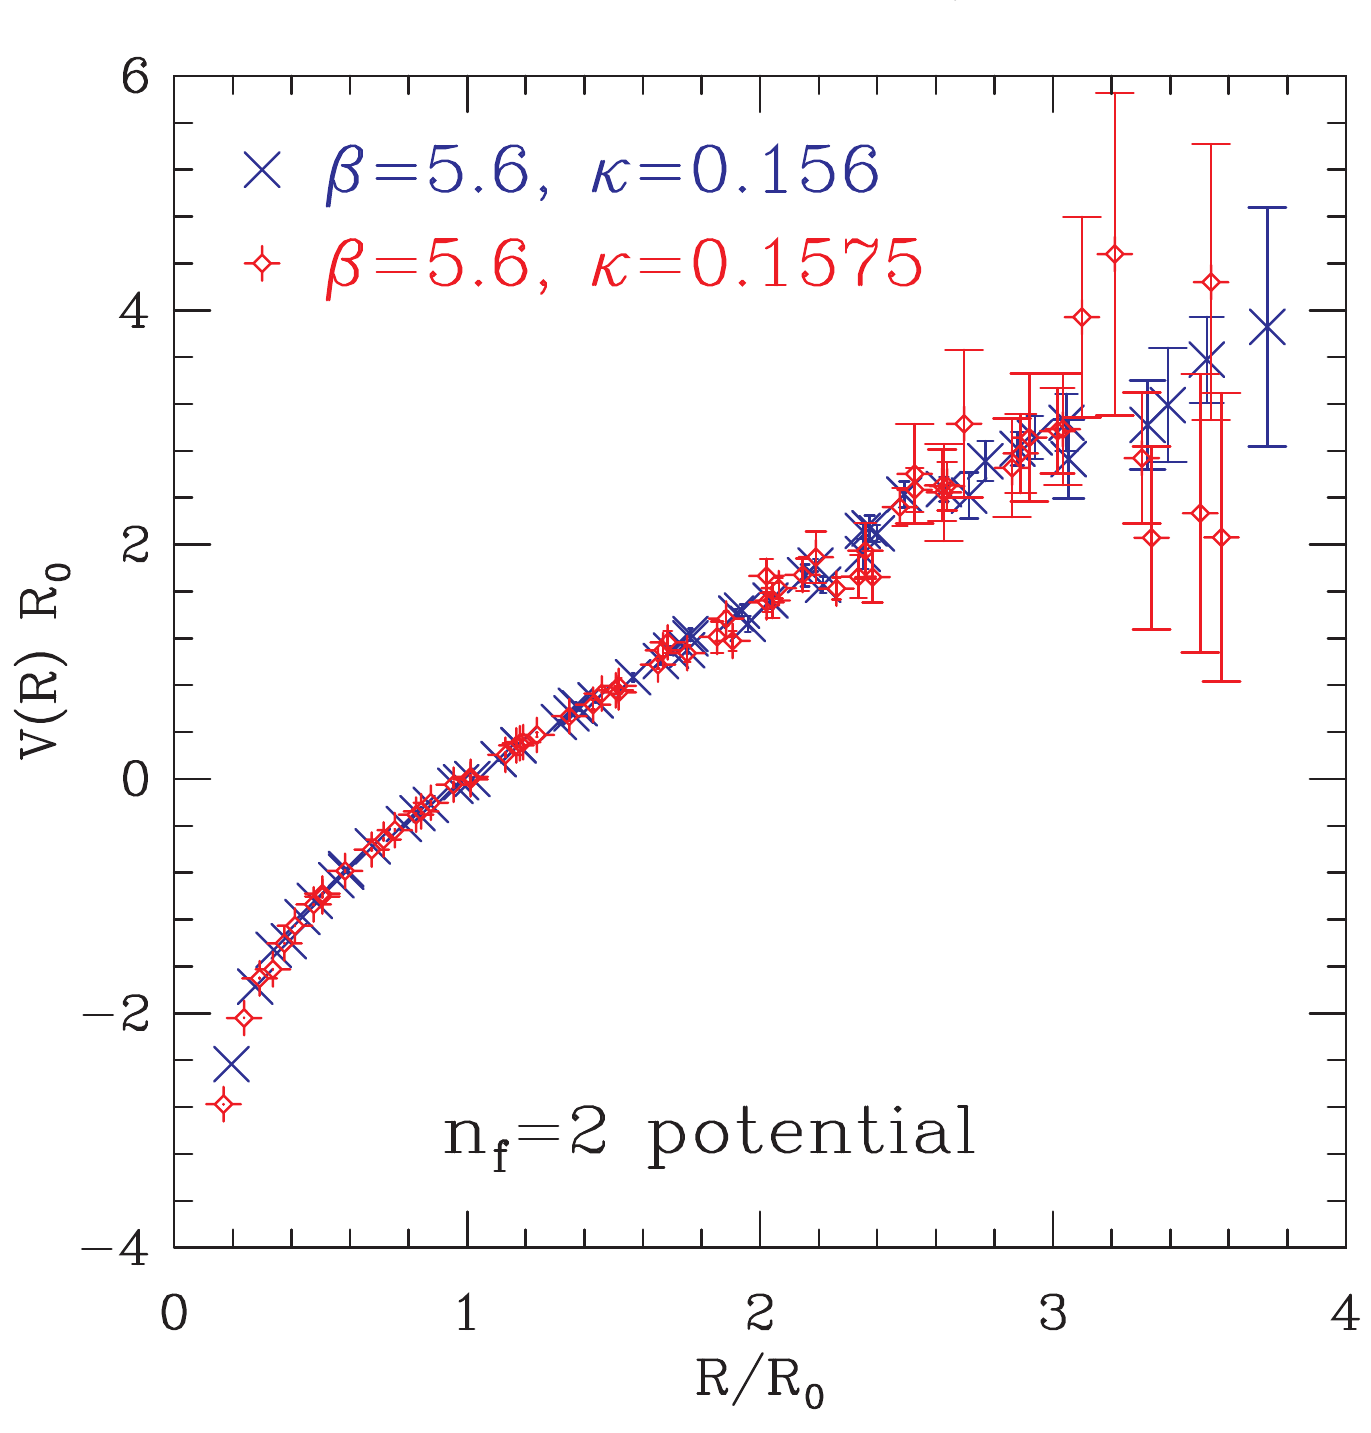
\includegraphics[width=0.8\textwidth]{images/fig11.png}
  \caption{The static $qq$ potential with two flavors of dynamical
    fermions obtained by the Wuppertal collaboration [119]. The dynamical
    quark mass in the $\beta = 6.0$, $\kappa = 0.156$ simulation is
    $\sim 2 m_s$ while that at $\kappa = 0.1575$ is $\sim m_s$. The rest is
    same as in Fig.~\ref{fig:10}. These data lie lower than the quenched
    points, however, for these dynamical quark masses there is no evidence
    yet of string breaking at large $R$.}
  \label{fig:11}
\end{figure}

The Cornell and Richardson potentials, which have been very successful in
predicting levels of charmonium and Upsilon system, yield
\begin{equation}
  R_0 \approx 0.49~\text{fermi}
  \label{eq:R0}
\end{equation}
Setting the scale using $R_0$ has the following advantages: (i) its value
is not very sensitive to the choice of the phenomenological potential,
(ii) it is defined at an intermediate distance where phenomenological
potentials are highly constrained by the $cc$ and $bb$ spectra,
(iii) lattice measurements of $V(R)$ at these intermediate distances can be
obtained with high precision, and (iv) this construction is valid for both
full and quenched QCD. The status of the current quenched data from three
collaborations is shown in Fig.~\ref{fig:12}. The data agree, and it turns
out that over this same range of $\beta$ the relation $R_0 = 1.18/\sqrt{\sigma}$
holds to a very good approximation. (The $\sigma$ is extracted from the
large $R$ behavior of the $qq$ potential as discussed above.) Thus, in
subsequent analyses of lattice data I will assume this relation when using
either $\sigma$ or $R_0$ to set the scale.

\begin{figure}[htbp]
  \centering
  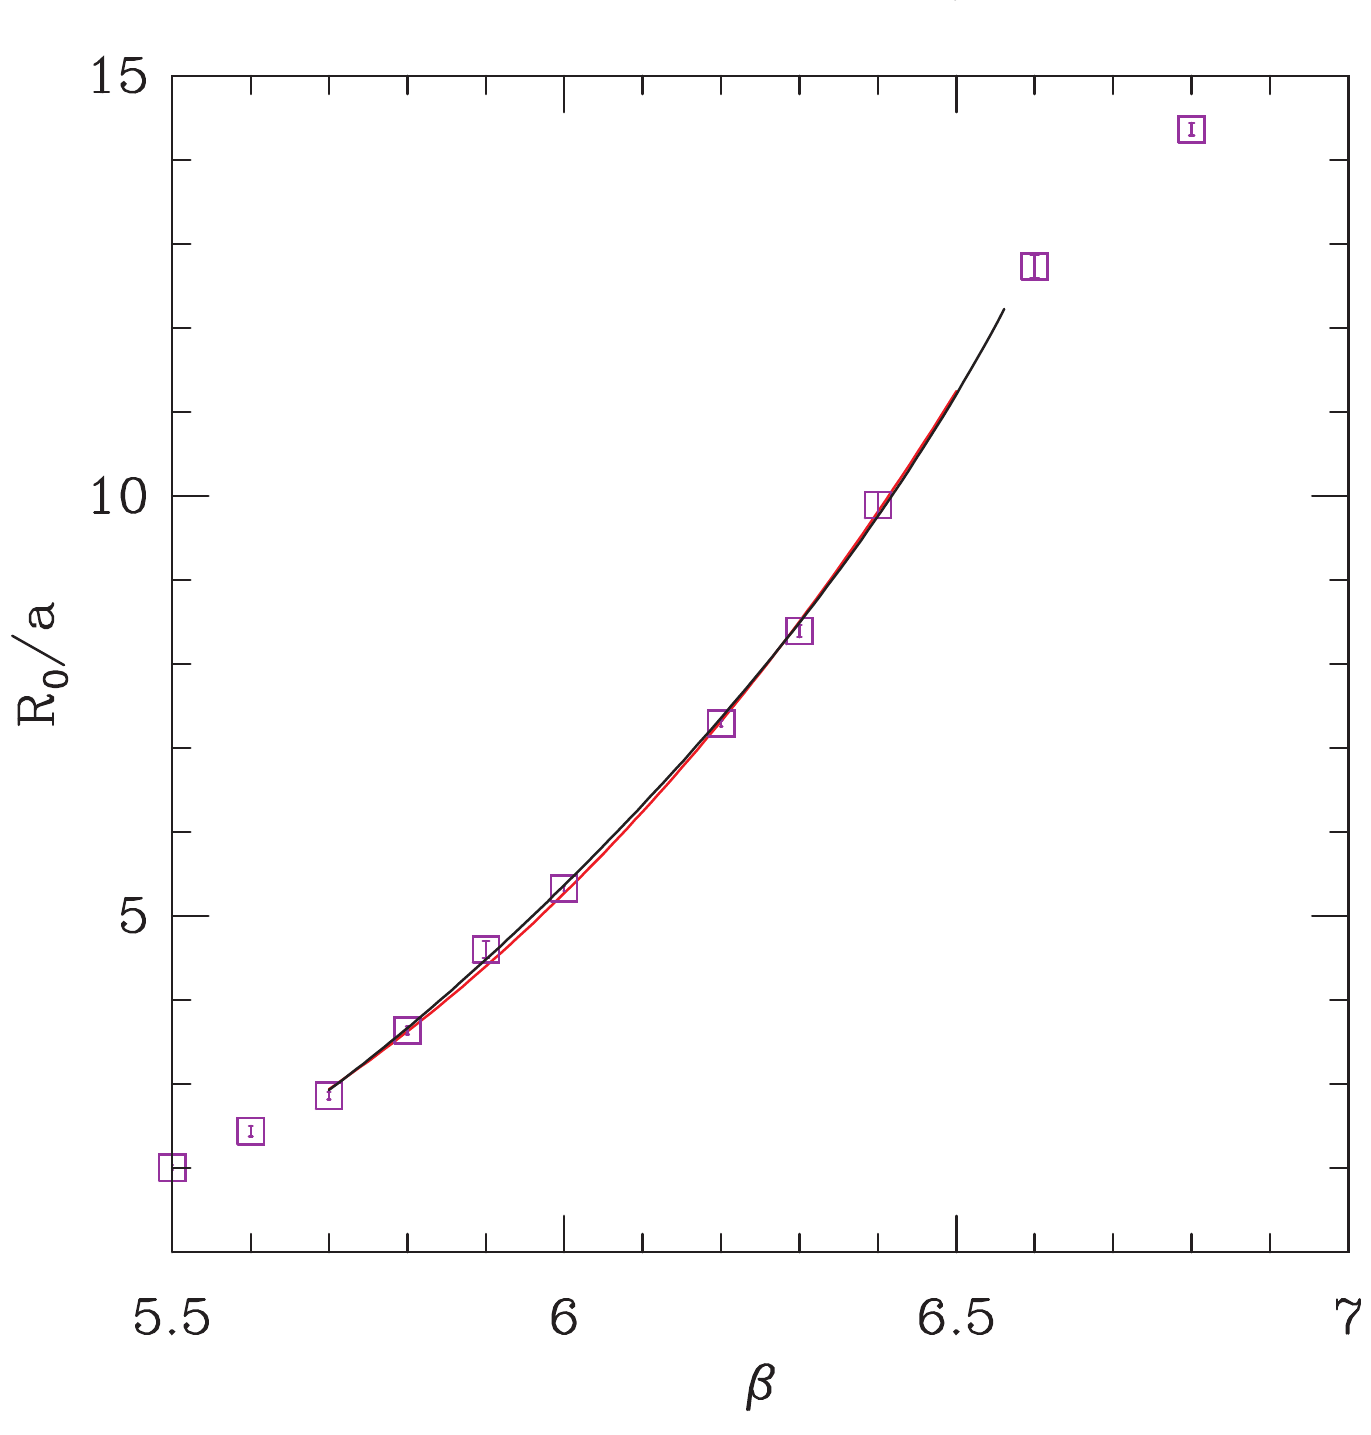
\includegraphics[width=0.8\textwidth]{images/fig12.png}
  \caption{The scale $R_0$ extracted from the static $qq$ potential. The
    data in purple are from [118,119,121] and the red line is a fit to
    these data. The black line is the fit
    $\log(a/R_0) = -1.6805 - 1.7139(\beta - 6) + 0.8155(\beta - 6.0)^2
    - 0.6667(\beta - 6)^3$ to the data by the Alpha collaboration [122].}
  \label{fig:12}
\end{figure}

For full QCD, the linear rising potential is screened. The string between
the $qq$ breaks when the energy is large enough to pop an additional $qq$
out of the vacuum and create two mesons. This phenomena of screening can
be tested by plotting $V(R)$ for different values of the dynamical quark
mass and observing the flattening of the linear rise. The value of $R/R_0$
at which the flattening should occur should decrease with $m_q$. A recent
analyses, again by the Wuppertal collaboration, is shown in
Fig.~\ref{fig:11} [119]. The data show no flattening---presumably because
the sea quark masses used in the update are not light enough to cause
string breaking at these $R/R_0$.

\subsection{Strong Coupling Expansion}
\label{sec:strong-coupling}

Confinement, for $\beta \to 0$, can be demonstrated using strong coupling
expansions. I will illustrate this technique by two examples---string
tension and the $0^{++}$ glueball mass.

The strong coupling expansion for SU($N$) gauge theory depends on the
following identities for integration over link matrices
\begin{align*}
  \int dg &= 1, &
  \int dg\, U_{ij} &= 0, &
  \int dg\, U_{ij}^\dagger &= 0, \\
  \int dg\, U_{ij} U_{kl} &= 0, &
  \int dg\, U_{ij}^\dagger U_{kl}^\dagger &= 0, &
  \int dg\, U_{ij} U_{kl}^\dagger &= \frac{1}{N}\delta_{il}\delta_{jk}
\end{align*}
\begin{equation}
  \int dg\, U_{i_1 j_1}\cdots U_{i_N j_N}
    = \frac{1}{N}\epsilon_{i_1\cdots i_N}\epsilon_{j_1\cdots j_N}.
  \label{eq:group-int}
\end{equation}
The essential point is that the group integration gives a non-zero result
only if each link occurs in a combination from which a color singlet can be
formed. Eq.~\eqref{eq:group-int} shows this for the identity, ``meson'' and
``baryon'' configuration of links.

The expectation value of the Wilson loop, at small $\beta$ (large $g$) for
the plaquette action, can be expanded as follows.
\begin{equation}
  \begin{aligned}
    W_{RT} &= \frac{1}{Z}\int dU\, W_{RT}\,
      e^{(\beta/2N)(W_{11}^{+}+W_{11}^{-})} \\
    &= \frac{1}{Z}\int dU\, W_{RT}\left[1 + \frac{\beta}{2N}\left(W_{11}^{+}
      + W_{11}^{-}\right) + \ldots\right]
  \end{aligned}
  \label{eq:W-expansion}
\end{equation}
where $W_{11}^{+}$, $W_{11}^{-}$ are the two orientations of the plaquette
and the trace over color incides in each loop is implicit. An inspection of
Fig.~\ref{fig:13}A shows that the first non-zero contribution to the
integral occurs when the loop $W_{RT}$ is tiled by elementary plaquettes
with the right orientation. Each such plaquette brings a factor of
$\beta/2N$ from the expansion and another factor of $1/N$ from the
integration. (Note that SU(2) is special and the combined factor is
$\beta/N^2$ as the two orientations of the loop have the same value, i.e.\
the trace is real.) Thus
\begin{equation}
  W_{RT} = \left(\frac{\beta}{2N^2}\right)^{RT}\left(1 + \ldots\right)
  \label{eq:W-area}
\end{equation}
where the leading corrections come from replacing any given tile with a
pillbox. Now using Eqs.~\eqref{eq:wilson-exp} and \eqref{eq:cornell} gives
\begin{equation}
  \sigma = -\log\frac{\beta}{2N^2} + O(\beta).
  \label{eq:sigma-sc}
\end{equation}
Thus all gauge theories, including U(1), confine in the strong coupling
limit. What distinguishes U(1) from non-abelian gauge theories is that the
U(1) gauge theory has a phase transition at $g^2 \sim 1$ (see
Section~15), and the physical theory
(electrodynamics) lies in the weak coupling region which is analytically
disconnected from the confining strong coupling limit.

As a second application of the strong coupling expansion consider the
calculation of $0^{++}$ glueball mass. The minimum tiling of the connected
plaquette-plaquette correlation function is the rectangular tube consisting
of four sides of size $1 \times T$ as shown in Fig.~\ref{fig:13}B. Thus
\begin{equation}
  W_{11}(T)W_{11}(0) \sim e^{-M_{0^{++}}T}
    = \left(\frac{\beta}{2N^2}\right)^{4T}\left(1 + \ldots\right),
  \label{eq:glueball}
\end{equation}
and
\begin{equation}
  M_{0^{++}} = -4\log\frac{\beta}{2N^2} + \ldots .
  \label{eq:Mglueball}
\end{equation}
The fact that the lowest order result $M_{0^{++}}/\sqrt{\sigma} = 4$ is very
close to present day estimates (see Section~18.3) is fortuitous.

\begin{figure}[htbp]
  \centering
  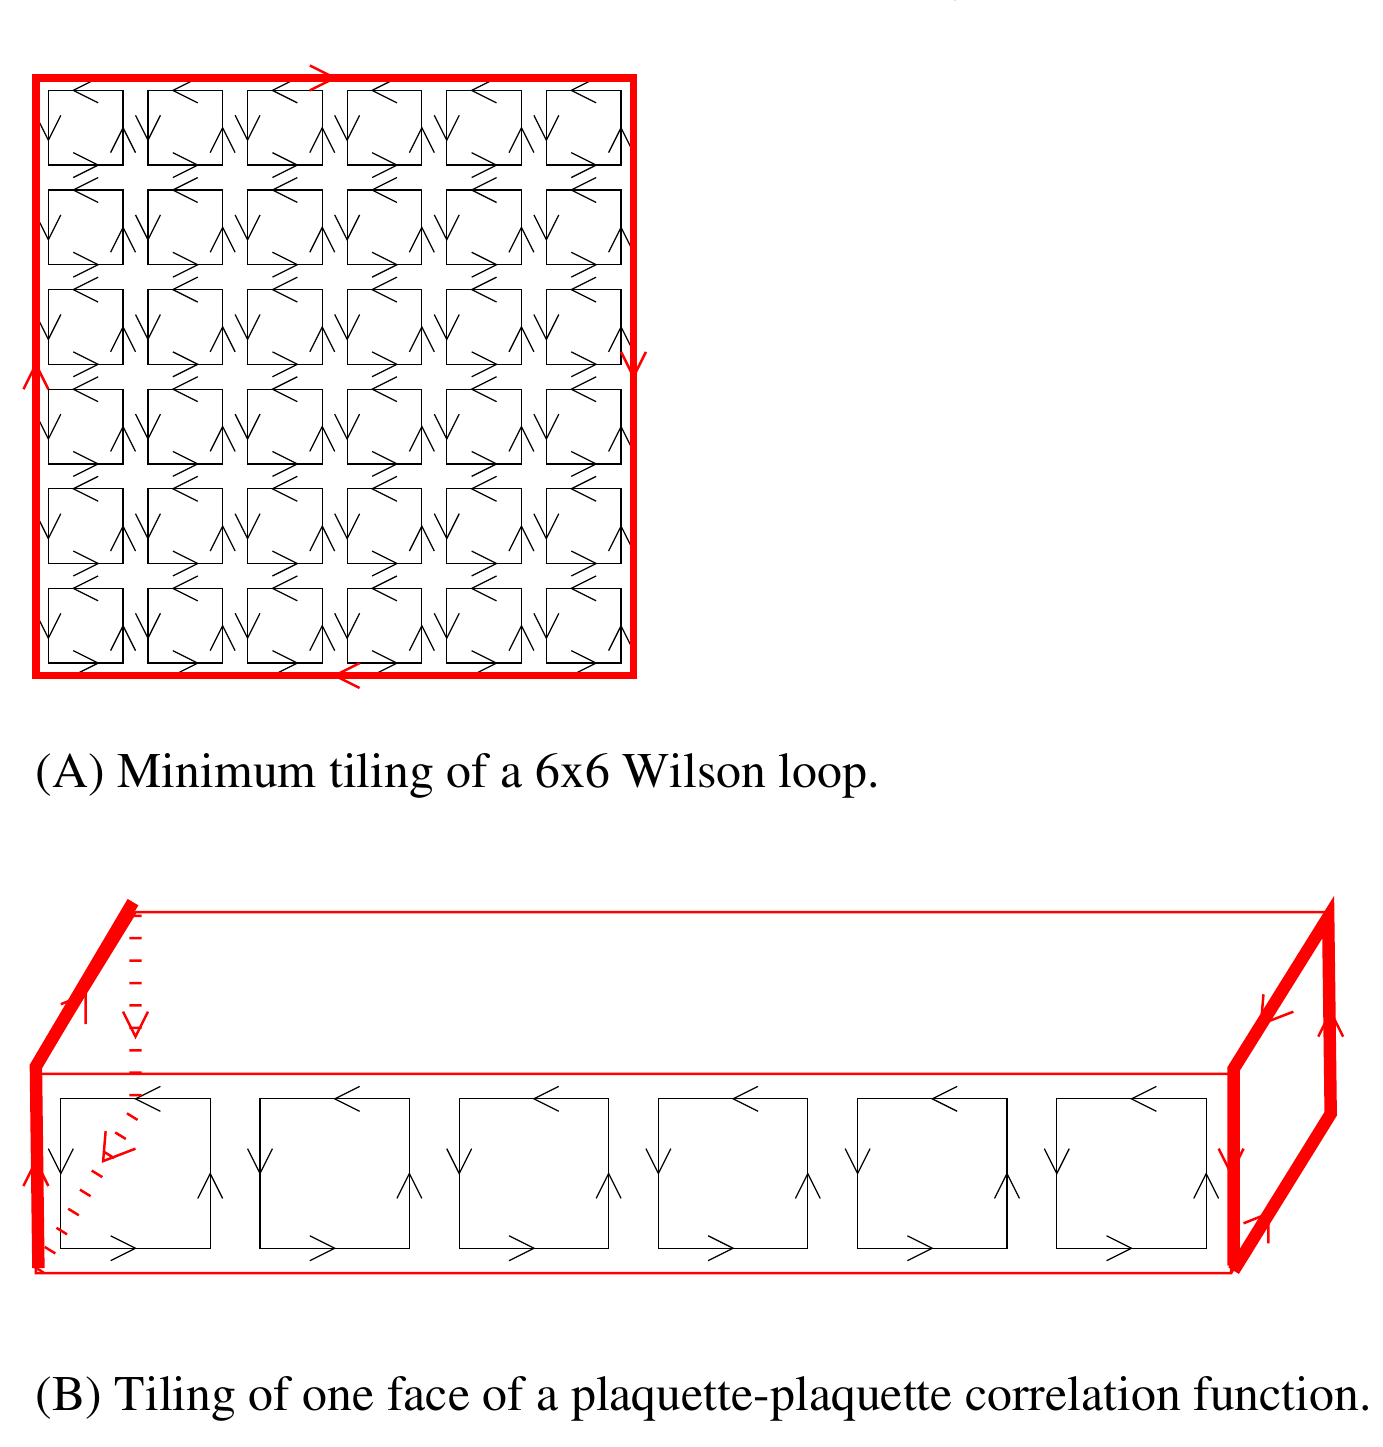
\includegraphics[width=0.8\textwidth]{images/fig13.png}
  \caption{Examples of minimum tiling of (A) a $6 \times 6$ Wilson loop,
    and (B) the plaquette-plaquette correlation function.}
  \label{fig:13}
\end{figure}

\textbf{Exercise:} What is the minimal tiling for the $0^{++}$ correlation
function built out of a $R \times R$ Wilson loop. Show that
Eq.~\eqref{eq:glueball} holds independent of the size of the loop.

\subsection{Wilson/Polyakov Line}
\label{sec:wilson-polyakov-line}

The Wilson line, pointing in say the time direction, is defined by the path
ordered product
\begin{equation}
  \langle L(x,y,z)\rangle = \mathrm{Tr}\, P \prod_{t=1}^{N_T}
    U_4(x,y,z,t)
  \label{eq:polyakov}
\end{equation}
It is gauge invariant due to periodic boundary conditions on gauge fields,
$U_4(x,y,z,N_T+1) = U_4(x,y,z,1)$. Repeating the above arguments made for
the Wilson loop one finds that the free energy of an isolated quark is
given by the Wilson/Polyakov line
\begin{equation}
  \langle L\rangle \sim e^{-F_q N_T}.
  \label{eq:free-energy}
\end{equation}
Thus, the possibility of having isolated charges in the theory requires
$F_q$ be finite.

In addition to gauge invariance, SU($N$) gauge theories have a global
$Z(N)$ invariance. It consists of multiplying all links on a given time
slice by the same element $z$ of $Z(N)$ without changing the action. Under
this transformation $\langle L\rangle \to z\langle L\rangle$. Such a global
symmetry can be spontaneously broken. Thus we have two possibilities
\begin{equation}
  \begin{array}{lll}
    \text{Broken:} & \langle L\rangle \neq 0 & \text{Deconfined}\ (F_q\ \text{finite}) \\
    \text{Unbroken:} & \langle L\rangle = 0 & \text{Confined}\ (F_q\ \text{infinite})
  \end{array}
  \label{eq:order-param}
\end{equation}
Thus, $\langle L\rangle$ is an order parameter, and tests for confinement
in pure gauge theories. It is also used to probe the location and order of
the finite temperature transition---a discontinuity in $\langle L\rangle$
signals a first order transition, whereas a continuous change implies
second order.

Svetitsky and Yaffe [128] argued that for the purposes of determining the
order of the finite temperature transition the relevant effective theory is
a 3-dimensional spin model of short-ranged interactions (between Wilson
lines reduced to spin variables) with a $Z(N)$ symmetry. Then using the
universality classes known from renormalization group analyses, they
predicted that the transition for SU(2) should be second order (Ising
class), whereas for SU($N \geq 3$) it should be first order (P\"otts
class). Numerical results are consistent with these predictions, in
particular for SU(2) the critical exponents have been determined using
standard techniques of Statistical Mechanics and found to agree with those
of the 3-dimensional Ising model [129].

In the presence of dynamical quarks, it is easy to see that the discretized
Dirac action is not invariant under the $Z(N)$ symmetry. Consequently,
$\langle L\rangle \neq 0$ for all values of $\beta$, so $\langle L\rangle$
is no longer an order parameter. Nevertheless, changes (discontinuous or
continuous) in it are used to search for the location of the finite
temperature phase transition and its order.
